\section{Evaluation}

We implement \spartacus in terms of Chrome extension, which the anti-phishing ecosystem can leverage and spread trivially.
and evaluate it from three perspectives, including effectiveness, user experience, and privacy.
These three aspects demonstrate the feasibility of the \spartacus system because it can successfully evade advanced phishing websites, can negligibly introduce latencies to the users when visiting websites, and can protect privacy of the users.

\subsection{Prevalence of Fingerprinting Cloaking}

\begin{figure}
\centering
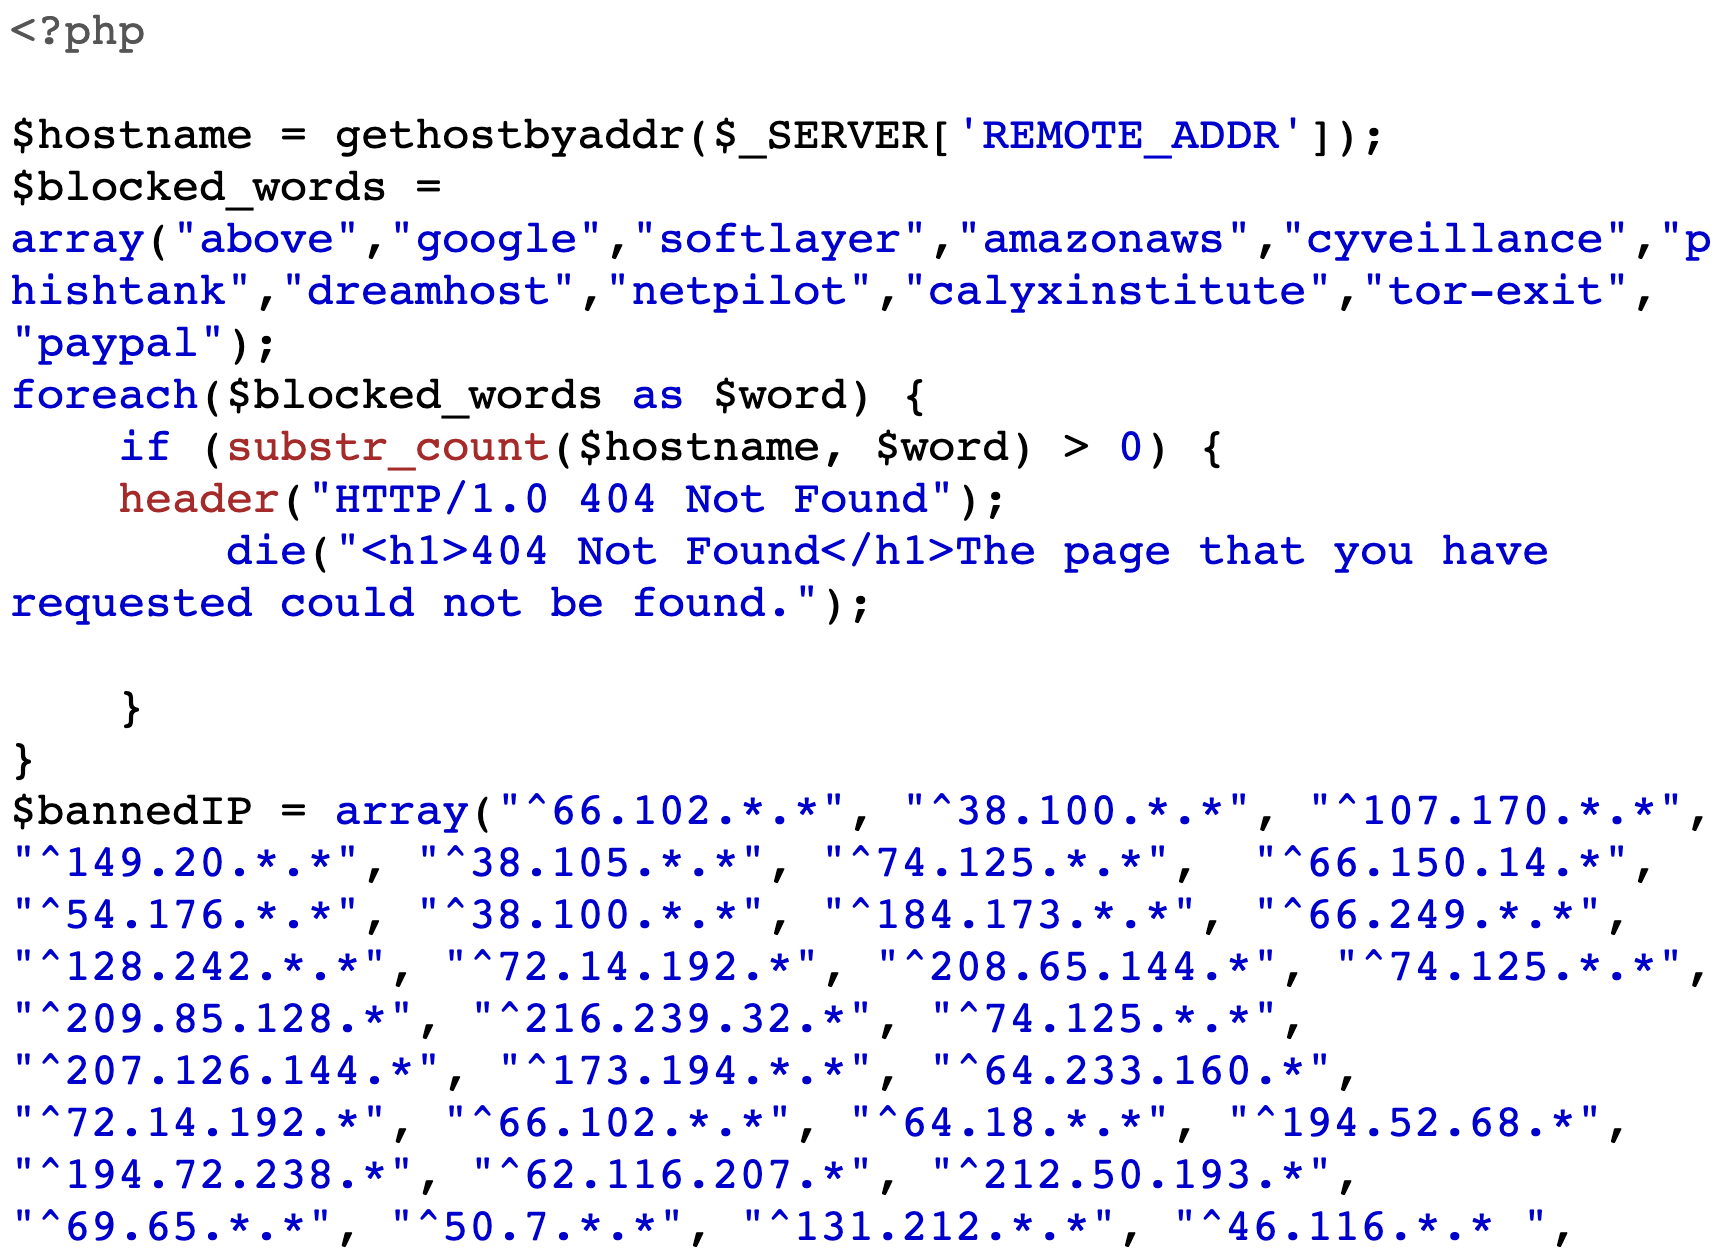
\includegraphics[width=\linewidth]{figs/server_cloaking.png}
\caption{PHP code snippet of fingerprinting cloaking in a phishing kit.}
\label{fig:servercloaking}
% \vspace{-10pt}
\end{figure}

To understand the prevalence of cloaking techniques used in advanced phishing kits, we manually inspect 56 phishing kits, and extract common patterns that implement fingerprinting cloaking techniques in phishing kits.

The patterns include (1) sensitive file names such as ``antibot'', ``blocker'', and ``antirobot''; (2) blocked words, for example, an array containing crawler information such as ``google'', ``paypal'', or ``phishtank'' (e.g., \texttt{blocked\_words} in~\autoref{fig:servercloaking}); (3) IP checker that blocks visit from certain IP addresses, such as \texttt{bannedIP} in~\autoref{fig:servercloaking}; and (4) error header, returning an error status code and an error web page, such as \texttt{header} function in PHP.
These attributes reflect the implementation of fingerprinting cloaking techniques in phishing kits.

With these patterns, we can automatically inspect such evasion to evaluate its prevalence.
Among the inspected kits in~\emph{phishunt.io}~\cite{phishunt} from January to June 2021, 198 of 236 contain cloaking techniques to fingerprint anti-phishing crawler visit through IP, Referrer, and/or User-Agent.
To comprehensively measure the prevalence of server-side fingerprinting cloaking techniques in phishing kits,
we also run our pattern finding script on Cisco's dataset that is contributed to Virus Total.
Preliminarily, 100 out of 100 phishing kits from Cisco's dataset contain such evasion.
% , while only one implements server-side click-through cloaking.

From this experiment,
we show that phishers prefer to fingerprint visit through information in HTTP request to distinguish humans out of crawlers.
And thanks to the fact, \spartacus can evade phishing websites generated from such advanced phishing kits.


% \subsection{Support From the Ecosystem}

% \spartacus focuses on the evasion of advanced phishing attacks,
% because the current anti-phishing techniques can effectively and efficiently detect and blacklist basic phishing~\cite{oest2020phishtime}.

% We still need to measure the ability of current anti-phishing systems against basic attacks.
% To this end, we submit phishing URLs to one of the systems, Google Safe Browsing (GSB), the same time when \spartacus inspects them.
% Meanwhile, we keep querying GSB for the blacklist result to calculate the blacklist speed.



\subsection{Effectiveness}

\begin{figure}[t]
    \centering
    \begin{subfigure}{0.48\linewidth}
        \centering
            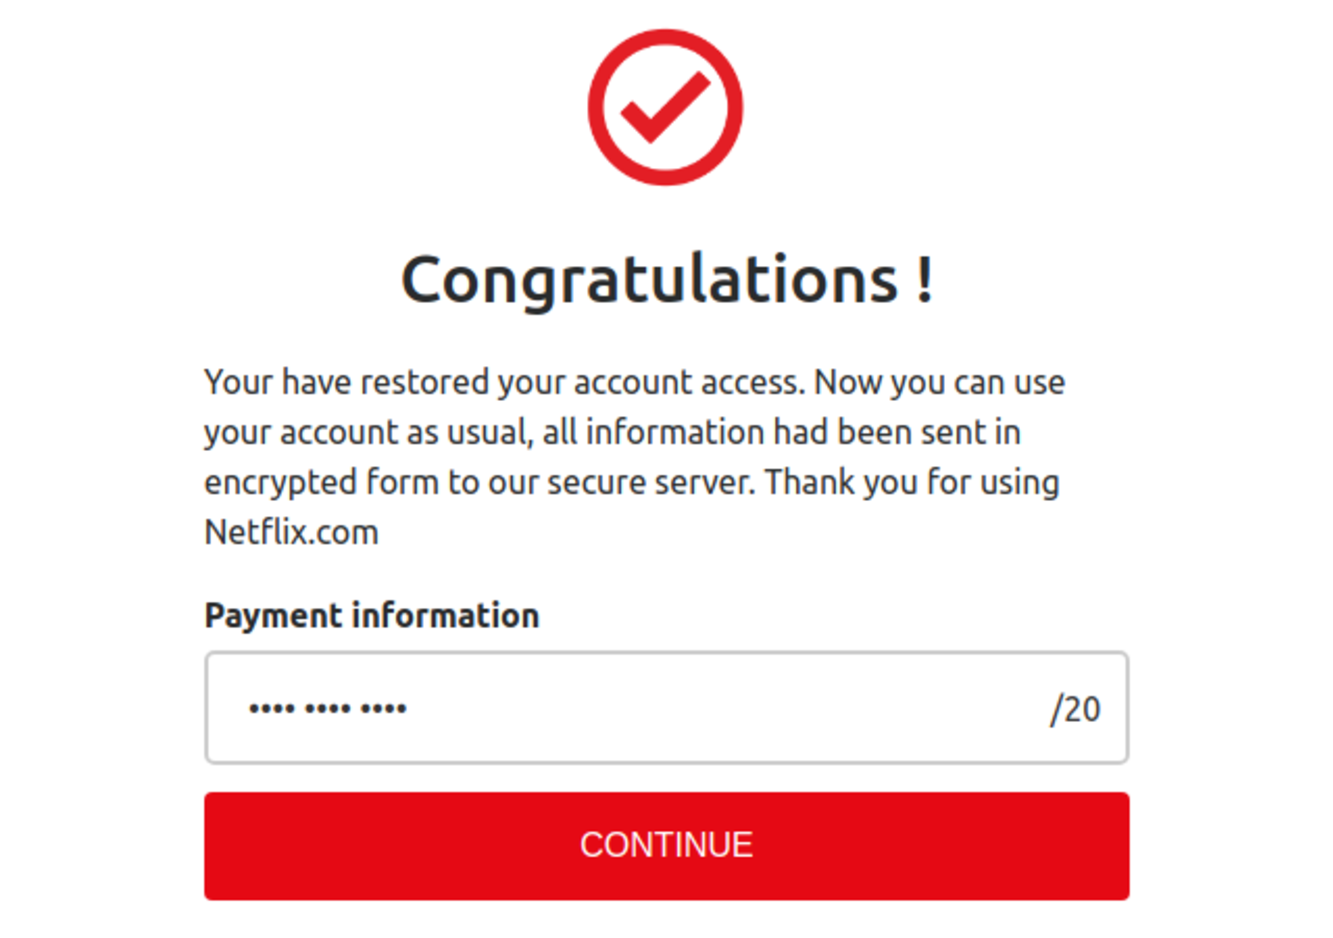
\includegraphics[width=\textwidth]{figs/netflix_n.pdf}%
        \caption{Default browser visit.}
        \label{fig:normal}
    \end{subfigure}
    ~
    \begin{subfigure}{0.48\linewidth}
        \centering
            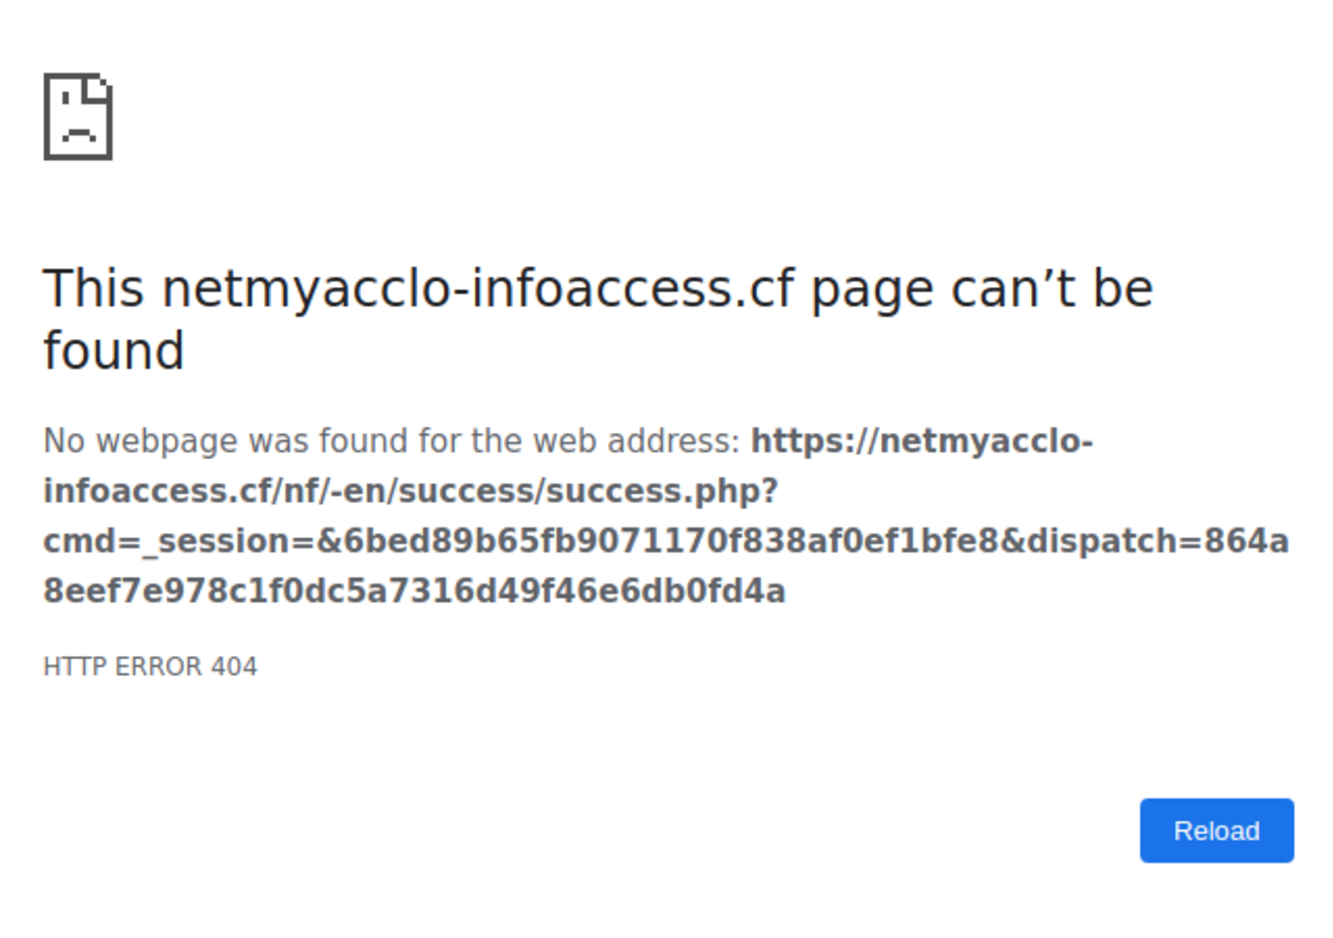
\includegraphics[width=\textwidth]{figs/netflix_sp.pdf}
        \caption{\spartacus visit.}
        \label{fig:sp}
    \end{subfigure}
    
    \caption{Web page contents from default and \spartacus'ed browser visits for a cloaked phishing website.}
    \label{fig:effectiveness}
    % \vspace{-10pt}
\end{figure}

We evaluate the effectiveness of \spartacus by conducting an experiment where we visit same phishing websites with different configurations of automated browsers, one with default setting, the other with \spartacus to mutate the profile.
We simulate the default setting automated browser as normal users and the one with \spartacus as users with our system.
The phishing URLs both browsers visit are from APWG, which is an open sourced dataset for reported phishing URLs.
For each visit, we record the final landing web page content and URL.
Either a legitimate final URL or a non-malicious web page content indicates the success of \spartacus evading phishing content for users.
If there is still malicious content shown to \spartacus, it indicates that either the phishing website does not contain advanced evasion techniques, or \spartacus does not trigger them with current fingerprint.
For the first situation, the current anti-phishing ecosystem has proposed methodologies to mitigate basic phishing attacks with effectiveness and efficiency.
As for the second, we believe that by visiting the same website with different configurations of HTTP requests mutated by \spartacus, the evasion techniques embedded in the phishing website can be triggered eventually. 

We examined 160,728 phishing URLs from APWG from November 2020 to July 2021,
132,247 of which do not contain malicious content.
We consider an HTTP response benign if (1) its web page content does not contain sensitive words or bad forms, according to CANTINA+~\cite{xiang2011cantina+};
(2) the response status code is an error one (4XX/5XX);
or (3) the destination domain is legitimate, excluding web hosting service domains.
\autoref{fig:effectiveness} demonstrates the difference of response web page content between default and \spartacus'ed browser visit for a cloaked phishing websites.
The content in~\autoref{fig:normal} shows the phishing content when a real person visits it.
On the other hand, when \spartacus appends a bot-looking string to the existing User-Agent, such as~\emph{googlebot}, the phishing server considers the visit as from an anti-phishing infrastructure.
Thus, it denies the request from \spartacus and an error web page is shown as~\autoref{fig:sp}.

It shows that \spartacus can impersonate anti-phishing crawler and trigger the cloaking techniques of advanced phishing websites.
Because the web page content returned through \spartacus's visit does not contain any maliciousness, Internet users will not be trapped in the attack.

% \textcolor{blue}{eval result}

\subsection{Support from Ecosystem}

Note that there are 17.72\% URLs that \spartacus cannot evade.
We hypothesize that these websites are basic phishing that do not contain cloaking techniques.
The anti-phishing systems nowadays such as Google Safe Browsing and VirusTotal can timely detect and/or blacklist traditional phishing attacks.
Therefore, they can handle the phishing websites that cannot be evaded by \spartacus.
And hence, \spartacus with the support of the anti-phishing ecosystem can prevent all types of phishing.

To verify our hypothesis, we evaluate the blacklist speed of current anti-phishing systems on the examined phishing URLs.
Due to the deployment of this experiment, we did not submit all phishing URLs.
Among 4,674 submitted phishing URLs, anti-phishing systems such as Google Safe Browsing and VirusTotal can blacklist 4,598 of them.
The median detection speed is 28 minutes.
The rest 76, after our manual inspection, is found that they are falsely reported to APWG.
The evaluation result verifies that the ecosystem currently can protect users from being trapped in basic phishing attacks.

In contrast, we totally submitted 47,885 URLs that can be evaded by \spartacus.
The result shows that 31,611 of them are not detected or blacklisted by the anti-phishing systems.
For URLs that can be detected, the median speed is 154 minutes, compared with that of 28 minutes for basic phishing websites.
Therefore, \spartacus not only can protect users from advanced phishing websites during the golden hour~\cite{oest2020sunrise} left by the current anti-phishing ecosystem due to process time, but also can evade phishing content even if the ecosystem cannot detect.


\subsection{Efficiency and Latency}

We need to make sure that \spartacus will not impact negatively on the user experience when they visit benign websites.
From the design of \spartacus, it will introduce latencies, including database query, HTTP profile mutation, and returned content inspection.
However, the latencies \spartacus introduces can be negligible.
Therefore, we conduct an experiment to measure the latency for the \spartacus system for the following three perspective, database query, profile mutation, and content inspection.
We leverage \emph{exthouse}, which analyzes the impact of a browser extension on web performance, as our test bench.
We run exthouse with 1,000 phishing websites and 1,000 benign websites on two configurations of browsers, one with \spartacus, the other without, and compare the mean rendering time for each group of websites.

\subsection{Impact on Benign Website}

Besides evading malicious content in phishing websites, \spartacus is also required to minimize the negative impacts on benign URL visit.
They can include ability of access the website, correct display of website layout, and correct functionalities of the website.
To evaluate the potential impacts to benign website, we conduct two experiments: Coarse-Grained and Fine-Grained.

\subsubsection{Coarse-Grained Experiment}

In Coarse-Grained experiment, we intend to evaluate if \spartacus system has negative impact on the access to the website or the website layout.
So we visit 60,848 (9.66\%) out of 629,843 URLs in Alexa Top One Million Domain List~\cite{AlexaTop1M} in both default and \spartacus'ed browsers.
We compare the web page screenshot and HTML similarity on the visited URLs.
Among them, 0.25\% (150) block the access from \spartacus'ed browser;
0.20\% (124) have different layouts.

To further differentiate between a legitimate anti-bot page and a phishing one that appears due to cloaking,
we extract domain reputation~\cite{reputation}, registration duration~\cite{whois}, and top viewed sub-domains~\cite{topviewedsubdomains} of URLs from false-positive (FP) and true-positive (TP) sides.
Cisco defines reputation of a domain as five categories: Trusted, Favorable, Neutral, Questionable, and Untrusted.
We inspect 150 URLs on each side.
Reputation-wise, 136 out of 150 TP URLs --- phishing --- have reputation lower or equal to Neutral level, the lowest of which is Poor Verdict.
In contrast, 24 of 150 FP URLs reside lower than Favorable level, the lowest of which is Questionable (only one).
In terms of domain lifespan, the mean value of domain duration since registration for FP URLs is 4,692 days and the median is 4,521 days.
However, the average lifespan of the malicious domains is 1,618 days, with median of 900 days.
Moreover, all 150 FP URLs fall into the top viewed sub-domains of the corresponding domain names, but none of the TP ones matches with them.

From the evaluation result, we summarize that a legitimate domain has a higher reputation and longer life than a malicious one, and they are within top viewed sub-domains.
With the finding, we can further reduce the FPs of \spartacus by querying the attributes of the domain to decide whether to mutate the HTTP profile.
We choose the phishing domain duration that resides on 75\% in the list (1,501) and Neutral level as threshold.
If one URL has a lifespan lower than 1,501 days and its reputation level is Neutral or worse, or its sub-domain is not top viewed, \spartacus will mutate the HTTP profile before request.
The logic is shown in~\Cref{alg:mutatelogic}.

\begin{algorithm}\captionsetup{labelfont={sc,bf}, labelsep=newline}
  \caption{Logic of mutating HTTP profile}
\begin{algorithmic}[1]

\State $p = default\_profile$
\State $u = url\_to\_visit$

\If{\State $reputation(u)~\leq Neutral$ \texttt{and}
\State $duration(u)~\geq 1,501$ \texttt{or} 
\State $d.domain$ NOT in top reviewed sub-domains}
    \State $p = mutate\_http\_profile(p)$
\EndIf

\State $send\_request(p)$

\end{algorithmic}
\label{alg:mutatelogic}
\end{algorithm}

We re-run the evaluation based on the threshold and find that 121 out of the 150 legitimate domains show same web page content on both default and \spartacus'ed browsers.
Hence, only 0.04\% of 60,848 domains are falsely evaded.
As comparison, all the phishing URLs can still be evaded through \spartacus because they all triggered the condition to invoke \emph{mutate\_http\_profile()}.

\subsubsection{Fine-Grained Experiment}

In Fine-Grained experiment, we aim to exercise and evaluate the operation of websites visited through \spartacus.
It was inspired by the methodology used by Snyder et al.~\cite{snyder2017most} and Trickel et al.~\cite{trickel2019everyone}.
This methodology concentrates on the operation of a website from the perspective of the user.
Even though \spartacus may introduce an error to a website while users do not perceive any difference when browsing, then we consider that \spartacus does not impact negatively on the website.
% evaluate potential impact \spartacus brings on the functionalities of benign domains.
This method of evaluation focuses more on potential impact \spartacus brings on the functionalities of benign domains than how \spartacus works.
And it was performed by the authors manually.

The experiment includes the evaluation of visibility of websites and interactions between visitor and the website.
It brings an additional metric that evaluates how \spartacus will influence users' daily activities.
There are four steps in the experiment.
(1) We open legitimate domains in a browser with \spartacus installed and also in one with default settings.
(2) We inspect the accessibility of the website, similar to the Coarse-Grained experiment.
(3) After the success of web page content retrieval, we compare the layouts between different visit.
(4) We interact with links, buttons, and other activities such as register/login, online chat, or shopping to make sure that their functionalities perform correctly.
(5) At last, we test the authentication functionality to make sure that \spartacus extension will not impact it.

We randomly selected 60 domains from Alexa Top One Million List, especially 20 every 200 thousands.
Among the 60 legitimate domains, we can access 58 of them.
Two domains are inaccessible even in the default browser, so we suspect them offline already.
For the accessible 58 domains,
we follow the steps mentioned above to inspect them.
All of them have the same layout as the visit from the default browser.


% \noindent
% \textbf{Database Query}.
% According to the e

% \noindent
% \textbf{Profile Mutation}.

% \noindent
% \textbf{Content Inspection}.

% \subsection{Privacy}

